\documentclass[10pt]{article}
\usepackage[a4paper,margin=2cm]{geometry}
\usepackage{graphicx}\graphicspath{{fig/}}
\usepackage{amsmath,amssymb}
\usepackage[dvipsnames,table]{xcolor}
\usepackage{booktabs,caption,enumitem}
\usepackage[colorlinks=true,urlcolor=accent,linkcolor=accent]{hyperref}
\usepackage{titlesec}
\definecolor{ink}{HTML}{201A40}\definecolor{accent}{HTML}{2563EB}
\definecolor{grn}{HTML}{0E6B4F}\definecolor{mut}{HTML}{55556A}
\definecolor{boxbg}{HTML}{F5F4FC}
\titleformat{\section}{\color{accent}\bfseries\large}{}{0pt}{}
\titlespacing{\section}{0pt}{11pt}{4pt}
\titleformat{\subsection}{\color{ink}\bfseries\normalsize}{}{0pt}{}
\titlespacing{\subsection}{0pt}{6pt}{2pt}
\setlist[itemize]{leftmargin=1.2em,itemsep=2pt,topsep=2pt}
\setlist[enumerate]{leftmargin=1.5em,itemsep=2pt,topsep=2pt}
\captionsetup{font={small,it},labelfont={color=mut},textfont={color=mut},skip=3pt}
\setlength{\parindent}{0pt}\setlength{\parskip}{4pt}\color{ink}\pagestyle{plain}
\newcommand{\keyword}[1]{\textbf{\color{accent}#1}}

\begin{document}

{\LARGE\bfseries HyMeKo: One Hypergraph Substrate for Representing and Learning from Structured Systems\par}
\vspace{2pt}{\color{accent}\itshape From declarative hypergraph structure to structural-prior learning.\par}
\vspace{1pt}{\color{mut}\small PhD Seminar~~$\cdot$~~Kato Laboratory~~$\cdot$~~Csaba Hajdu~~$\cdot$~~June 2026~~$\cdot$~~\emph{a primer-style handout: it starts from basic graph theory}\par}
\vspace{4pt}\hrule\vspace{6pt}

\section*{\color{accent}1.\quad Introduction --- why graphs, and why that is not enough}
Much of the world is naturally described by \keyword{relations between things}: people who trust or distrust each other, joints connected in a robot, atoms bonded in a molecule, layers wired in a neural network. The standard tool for relations is a \emph{graph}: dots (\emph{vertices}) joined by lines (\emph{edges}). Graphs are everywhere because they are simple and well understood.

But an ordinary edge joins \emph{exactly two} vertices, and many real relations are \keyword{$n$-ary} --- they bind several things at once. ``Alice, Bob and Carol co-authored a paper'' is one three-way fact, not three separate pairwise friendships. If we force it into a graph we draw three edges (Figure~\ref{fig:pvg}, left) and silently lose the information that it was \emph{one} joint event. A \keyword{hypergraph} keeps it as a single \emph{hyperedge} that contains all three (Figure~\ref{fig:pvg}, right).

This talk follows one idea through to its consequences. We take the hypergraph seriously as the basic object and ask two questions about it: (i) \emph{how do we describe} a structured system so that one description can drive many tools (simulators, robot formats, modelling languages, tensor libraries)? and (ii) \emph{how do we learn} from that same structure? HyMeKo answers both with a single substrate --- \emph{the structure the framework compiles is the structure the model reasons over}.

\begin{figure}[h]\centering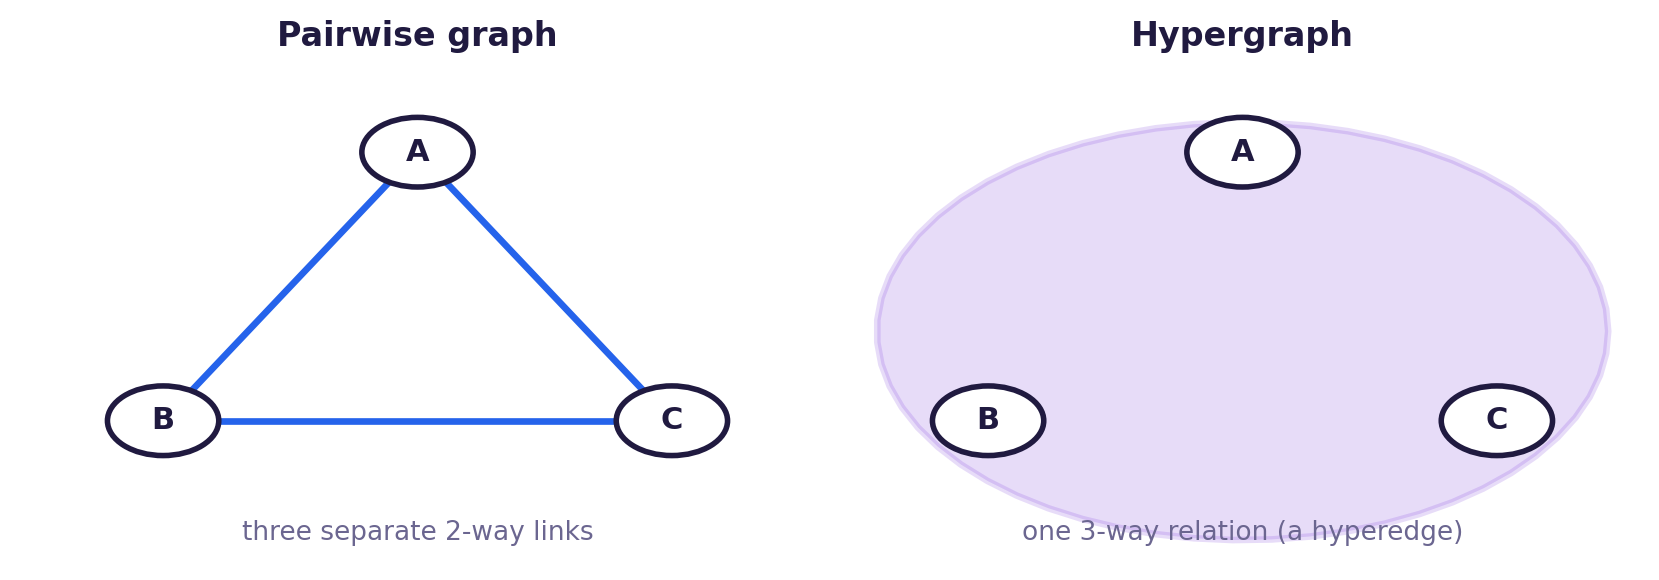
\includegraphics[width=.74\linewidth]{pairwise_vs_group.png}
\caption{A pairwise graph records three 2-way links; a hypergraph records one 3-way relation. Pairwise encodings lose the identity of group relations.}\label{fig:pvg}\end{figure}

\section*{\color{accent}2.\quad A short tour of graph theory (from the basics)}
\subsection*{Vertices, edges, neighbours, degree}
A \keyword{graph} is a pair $G=(V,E)$: a set of \keyword{vertices} (nodes) $V$ and a set of \keyword{edges} $E$, where each edge $\{u,v\}$ joins two vertices. If edges have a direction we write $(u\!\to\! v)$ and call the graph \emph{directed}. The \keyword{neighbours} of a vertex $v$ are the vertices joined to it, $N(v)$, and its \keyword{degree} is $\deg(v)=|N(v)|$ --- how many connections it has. In Figure~\ref{fig:basic}, $\deg(B)=3$ (neighbours $A,C,D$).

\subsection*{Walks, paths and cycles}
A \keyword{walk} is a sequence of edges followed end-to-end, e.g.\ $A\!-\!B\!-\!C$; its \emph{length} is the number of edges. A \keyword{path} is a walk that never repeats a vertex. A \keyword{cycle} is a closed path that returns to where it started, e.g.\ $A\!-\!B\!-\!D\!-\!E\!-\!A$. These three notions --- walk, path, cycle --- are central later: HyMeKo's models read structure off the \emph{cycles} of a graph.

\subsection*{Two matrices that store a graph}
With $n=|V|$ vertices and $m=|E|$ edges, a graph is stored either as an \keyword{adjacency matrix} $A\in\{0,1\}^{n\times n}$ (with $A_{ij}=1$ when $i,j$ are joined) or as an \keyword{incidence matrix} $B\in\{0,1\}^{n\times m}$ (with $B_{ie}=1$ when vertex $i$ belongs to edge $e$). Edges may also carry a \keyword{weight} (a number) or, as we use next, a \keyword{sign}.

\begin{figure}[h]\centering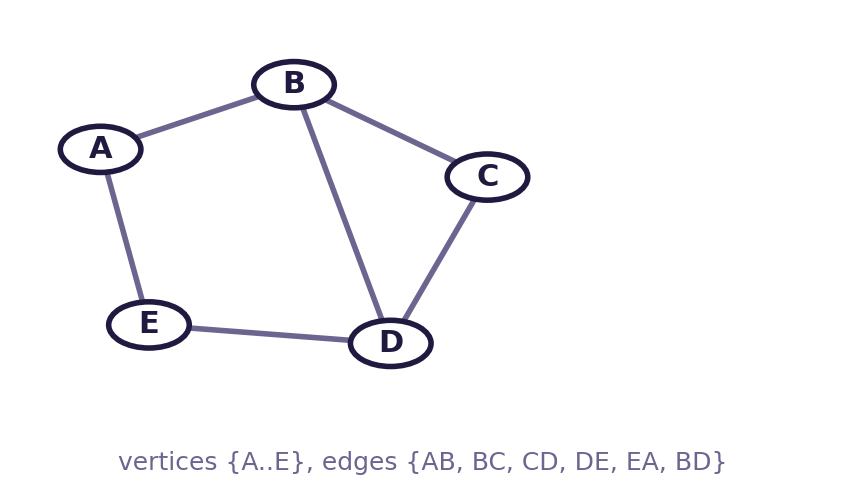
\includegraphics[width=.50\linewidth]{basic_graph.png}
\caption{A small undirected graph. Example path $A\!-\!B\!-\!C$; example cycle $A\!-\!B\!-\!D\!-\!E\!-\!A$; $\deg(B)=3$.}\label{fig:basic}\end{figure}

\subsection*{A few more kinds of graph}
Several special shapes recur. A graph is \keyword{complete} ($K_n$) when every pair of vertices is joined --- it has $\binom{n}{2}$ edges, the densest case. It is \keyword{bipartite} when the vertices split into two sides with edges only \emph{across} (never within) a side; the signed ``star'' form of a hyperedge ($\S6$) is exactly a bipartite graph. A \keyword{tree} is a connected graph with no cycles; on $n$ vertices it has exactly $n-1$ edges, the sparsest connected case. A \keyword{subgraph} keeps a subset of the vertices and edges. Edges may also be \keyword{directed} (an arc $u\!\to\!v$, as in dataflow or a kinematic chain) or \keyword{weighted} (a number per edge); the \keyword{sign} we use next is the simplest weight, just $\pm1$.

\subsection*{Connectivity, distance, and the Laplacian}
Two vertices are \keyword{connected} if some walk joins them, and a maximal connected piece is a \keyword{component}. The \keyword{distance} between two vertices is the length of a shortest path between them, and the largest such distance is the graph's \keyword{diameter}. Collecting the degrees on a diagonal gives the \keyword{degree matrix} $D$, and $L=D-A$ is the \keyword{graph Laplacian} --- the discrete analogue of a second derivative, whose spectrum encodes how connected and how ``smooth'' the graph is. The Laplacian, and its higher-order Hodge relatives, returns later: it is how the vision variant measures curvature and flow over a hypergraph.

\section*{\color{accent}3.\quad Signed graphs \& structural balance}
A \keyword{signed graph} adds a sign to every edge, $\sigma:E\to\{+,-\}$ --- think trust/distrust, friend/foe, agreement/disagreement. Structural balance is \emph{not} part of a standard first graph-theory course, so we spell it out.

\textbf{The triangle cases.} Take three people and the relationships among them. Up to relabelling there are four sign patterns (Figure~\ref{fig:triads}): all-positive ($+\!+\!+$), two-positive-one-negative ($+\!+\!-$), one-positive-two-negative ($+\!-\!-$), and all-negative ($-\!-\!-$). A triangle is \keyword{balanced} when the \emph{product} of its three edge signs is $+$. This matches social intuition (Heider, 1946): ``a friend of my friend is a friend'' ($+\!+\!+$) and ``an enemy of my enemy is a friend'' ($+\!-\!-$) are the comfortable, balanced cases, whereas ``a friend of my friend is my enemy'' ($+\!+\!-$) and ``three mutual enemies'' ($-\!-\!-$) feel tense and are unbalanced.

\textbf{From triangles to any cycle.} The same rule extends to every cycle: $\sigma(C)=\prod_{e\in C}\sigma(e)$, and $C$ is balanced iff this product is $+$.

\textbf{Harary's balance theorem (1953).} A signed graph is \emph{fully} balanced exactly when its vertices can be split into two camps so that every $+$ edge stays \emph{within} a camp and every $-$ edge runs \emph{between} them --- ``two factions: friends inside, enemies across.''

\textbf{Weak balance, and how balanced real graphs are.} Heider's original notion (1946) was psychological; Cartwright and Harary (1956) gave it the graph-theoretic form above. Davis (1967) then relaxed it: a graph is \keyword{weakly balanced} (\emph{clusterable}) when no cycle has \emph{exactly one} negative edge --- which permits all-negative triangles (three mutual rivals in three different camps) and lets the vertices fall into $k\ge2$ camps, not only two. No real social or trust network is perfectly balanced; the standard measure of how far off it is, is the \keyword{frustration (line) index} --- the fewest edge-sign flips needed to reach balance. Empirically these networks sit close to balance, and that closeness is exactly what makes the missing-sign question answerable at all.

\textbf{Why this drives prediction.} Real networks are only \emph{approximately} balanced, but the pull toward balance is strong, so the sign of a \emph{missing} edge is usually the one that keeps the cycles through it balanced. \keyword{Signed link-sign prediction} hides some edge signs and asks a model to recover them; HSiKAN and G\"omb learn a soft, data-driven version of exactly this cycle-balance signal --- and doing it \emph{honestly}, without peeking at the answer through the structure, is a recurring theme of the talk.


\begin{figure}[h]\centering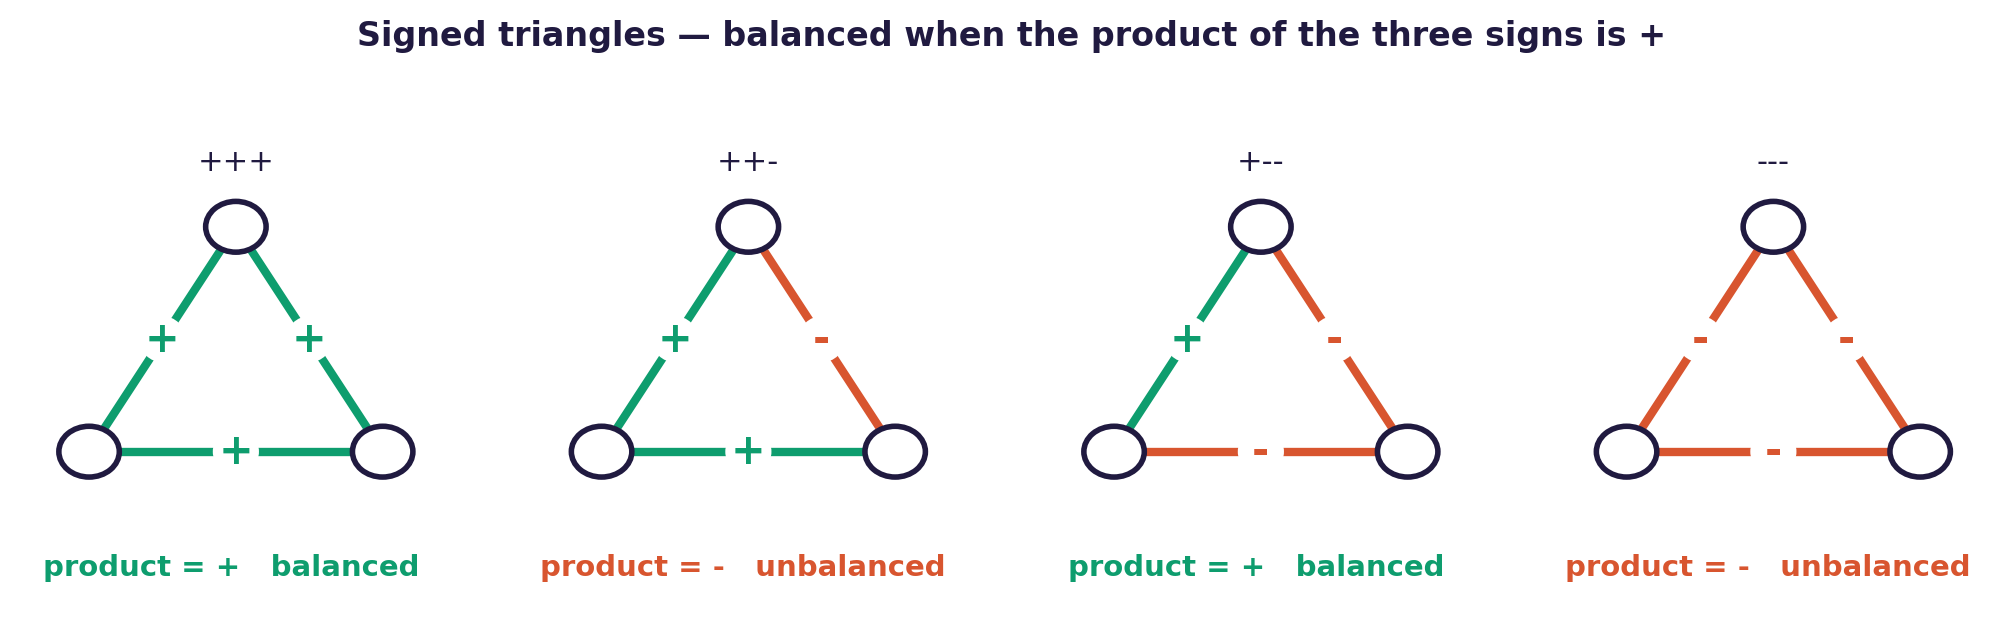
\includegraphics[width=.92\linewidth]{balance_triads.png}
\caption{The four signed triangles. Balanced $\Leftrightarrow$ the product of the three edge signs is $+$ (the $+\!+\!+$ and $+\!-\!-$ cases); the other two are unbalanced.}\label{fig:triads}\end{figure}

\begin{figure}[h]\centering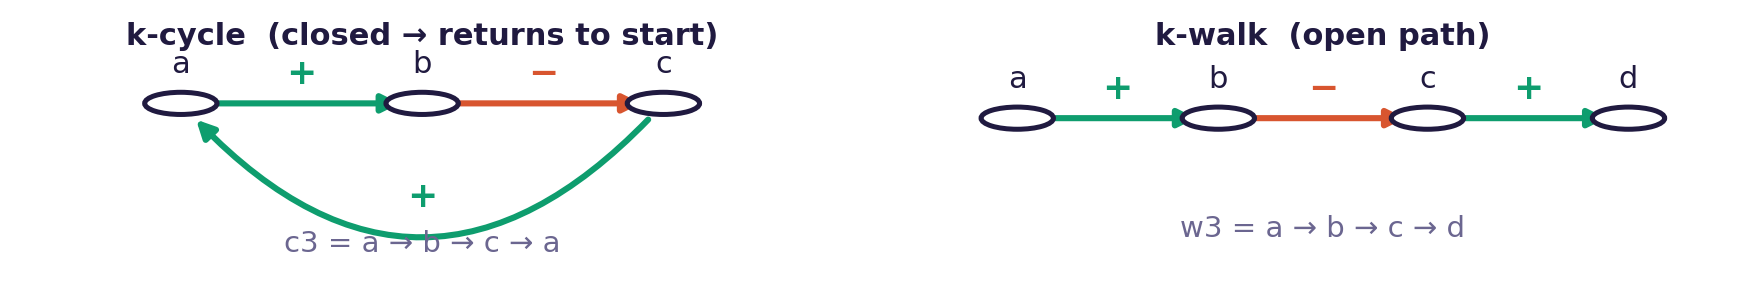
\includegraphics[width=.80\linewidth]{kcw.png}
\caption{A $k$-cycle (closed: returns to its start) and a $k$-walk (open path); green $+$, red $-$. A cycle's sign is the product of its edge signs.}\end{figure}

\section*{\color{accent}4.\quad From graphs to hypergraphs}
A \keyword{hypergraph} $H=(V,E)$ relaxes the ``two endpoints'' rule: each \keyword{hyperedge} $e\in E$ is simply a subset of vertices, $e\subseteq V$, of any size $|e|=k$ (its \emph{arity}). $k=2$ recovers an ordinary graph; $\bar d$ denotes the mean arity. Two standard ways turn a hypergraph back into something a matrix library can chew on:
\begin{itemize}
\item \keyword{Star (Levi/Berge) expansion.} Add one ``hub'' node per hyperedge and connect it to that hyperedge's members; the signed vertex$\times$hyperedge incidence is $B\in\{-1,0,+1\}^{|V|\times|E|}$. Cost is \keyword{$O(|E|\,\bar d)$} --- linear in the arity.
\item \keyword{Clique expansion.} Replace each hyperedge by a clique (join all its members pairwise). This recovers a plain graph but costs \keyword{$O(|E|\,\bar d^{2})$} --- the quadratic ``blow-up'' (a $k$-way relation becomes $\binom{k}{2}$ edges).
\end{itemize}
HyMeKo uses the star expansion precisely to keep cost linear and to preserve each relation's identity (Figure~\ref{fig:levi}).

\begin{figure}[h]\centering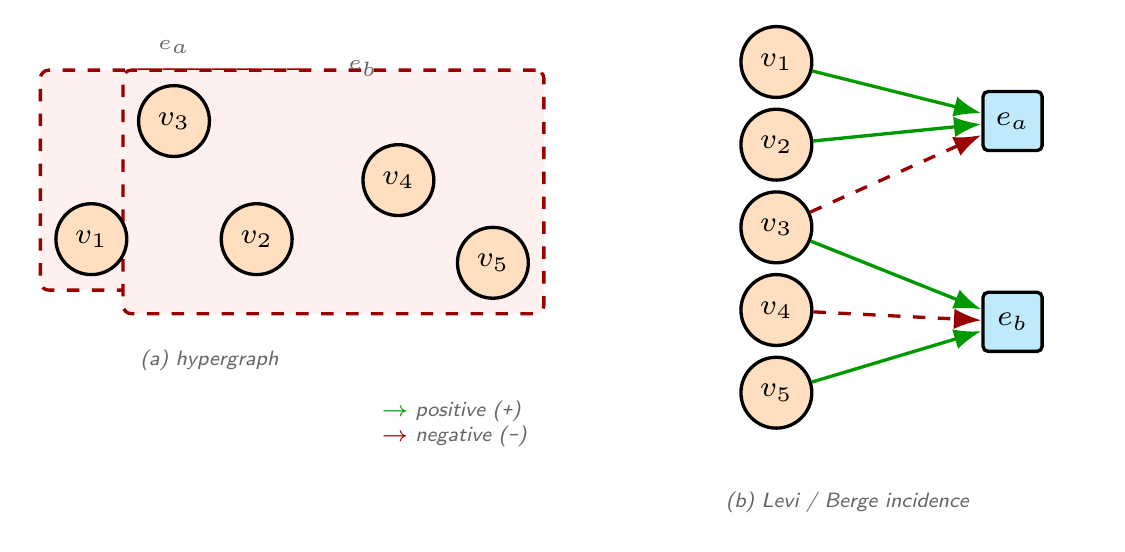
\includegraphics[width=.62\linewidth]{levi.png}
\caption{A signed hypergraph (hyperedges $e_a,e_b$ over $v_1\dots v_5$) and its Levi/Berge incidence --- the star expansion (green $+$, red $-$).}\label{fig:levi}\end{figure}

\section*{\color{accent}5.\quad Kolmogorov--Arnold representation \& KANs}
A classical theorem (Kolmogorov--Arnold, 1957) says any continuous function of many variables can be written using only \emph{single-variable} functions and addition:
\[ f(x_1,\dots,x_n)=\sum_{q=0}^{2n}\Phi_q\!\Big(\sum_{p=1}^{n}\psi_{q,p}(x_p)\Big). \]
A \keyword{Kolmogorov--Arnold Network (KAN)} turns this into a learnable model: instead of fixed activations (like ReLU) on the \emph{nodes}, it places \emph{learnable single-variable functions on the edges}. We represent each such function as a \keyword{spline} --- a smooth curve pinned to a few control points (here a Catmull--Rom spline, Figure~\ref{fig:cr}). HSiKAN puts these learnable splines on the \emph{signed cycle and walk tuples} of the hypergraph, so the graph's own structure becomes the model's inductive prior.

Why is the theorem surprising? It says the only genuinely multivariate operation you ever need is \emph{addition}: all the ``shape'' lives in one-dimensional functions $\psi_{q,p}$ and $\Phi_q$. A KAN takes that literally. A conventional \keyword{MLP} fixes the activation (ReLU, tanh) and \emph{learns the linear weights} on its edges; a KAN inverts this --- the edges carry the \emph{learnable functions}, and there is no separate weight matrix. A function's parameters are just the heights of a handful of \keyword{control points}, and a \keyword{Catmull--Rom} spline interpolates smoothly \emph{through} those points with local control (moving one point only perturbs its neighbourhood), so the curve stays interpretable and cheap to evaluate.

This is a good fit for our setting. A signed cycle's contribution is a fairly smooth function of its tuple of features, and we would rather the model \emph{learn which cycle lengths matter} than assume it in advance. Placing one learnable spline per signed cycle/walk tuple makes the graph's own structure the inductive prior --- the model's capacity is spent on the shape of the structure-to-sign map, not on a generic dense network.

\begin{figure}[h]\centering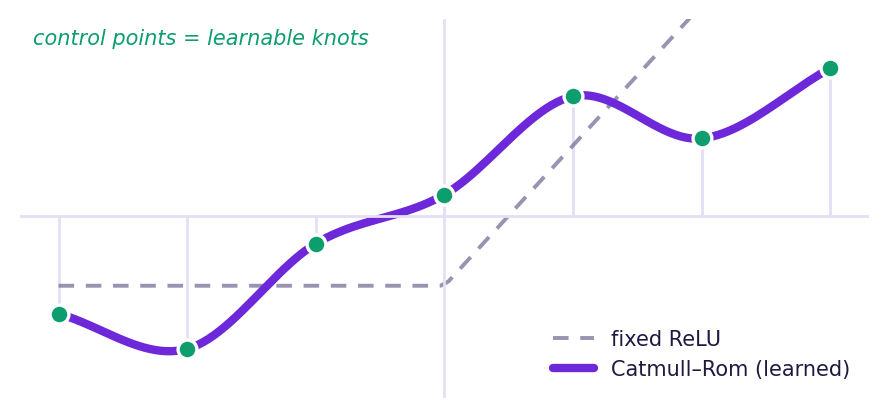
\includegraphics[width=.40\linewidth]{cr.png}
\caption{A learnable Catmull--Rom spline activation (vs.\ a fixed ReLU) --- the KAN primitive.}\label{fig:cr}\end{figure}

\section*{\color{accent}6.\quad One substrate, two payoffs}
A declarative \texttt{.hymeko} source compiles through a SIMD lexer and an LALRPOP parser to one canonical hypergraph IR with a Blake3 content-hash identity. From that single IR the framework both emits many target formats and feeds the structural-prior learning stack.

\begin{figure}[h]\centering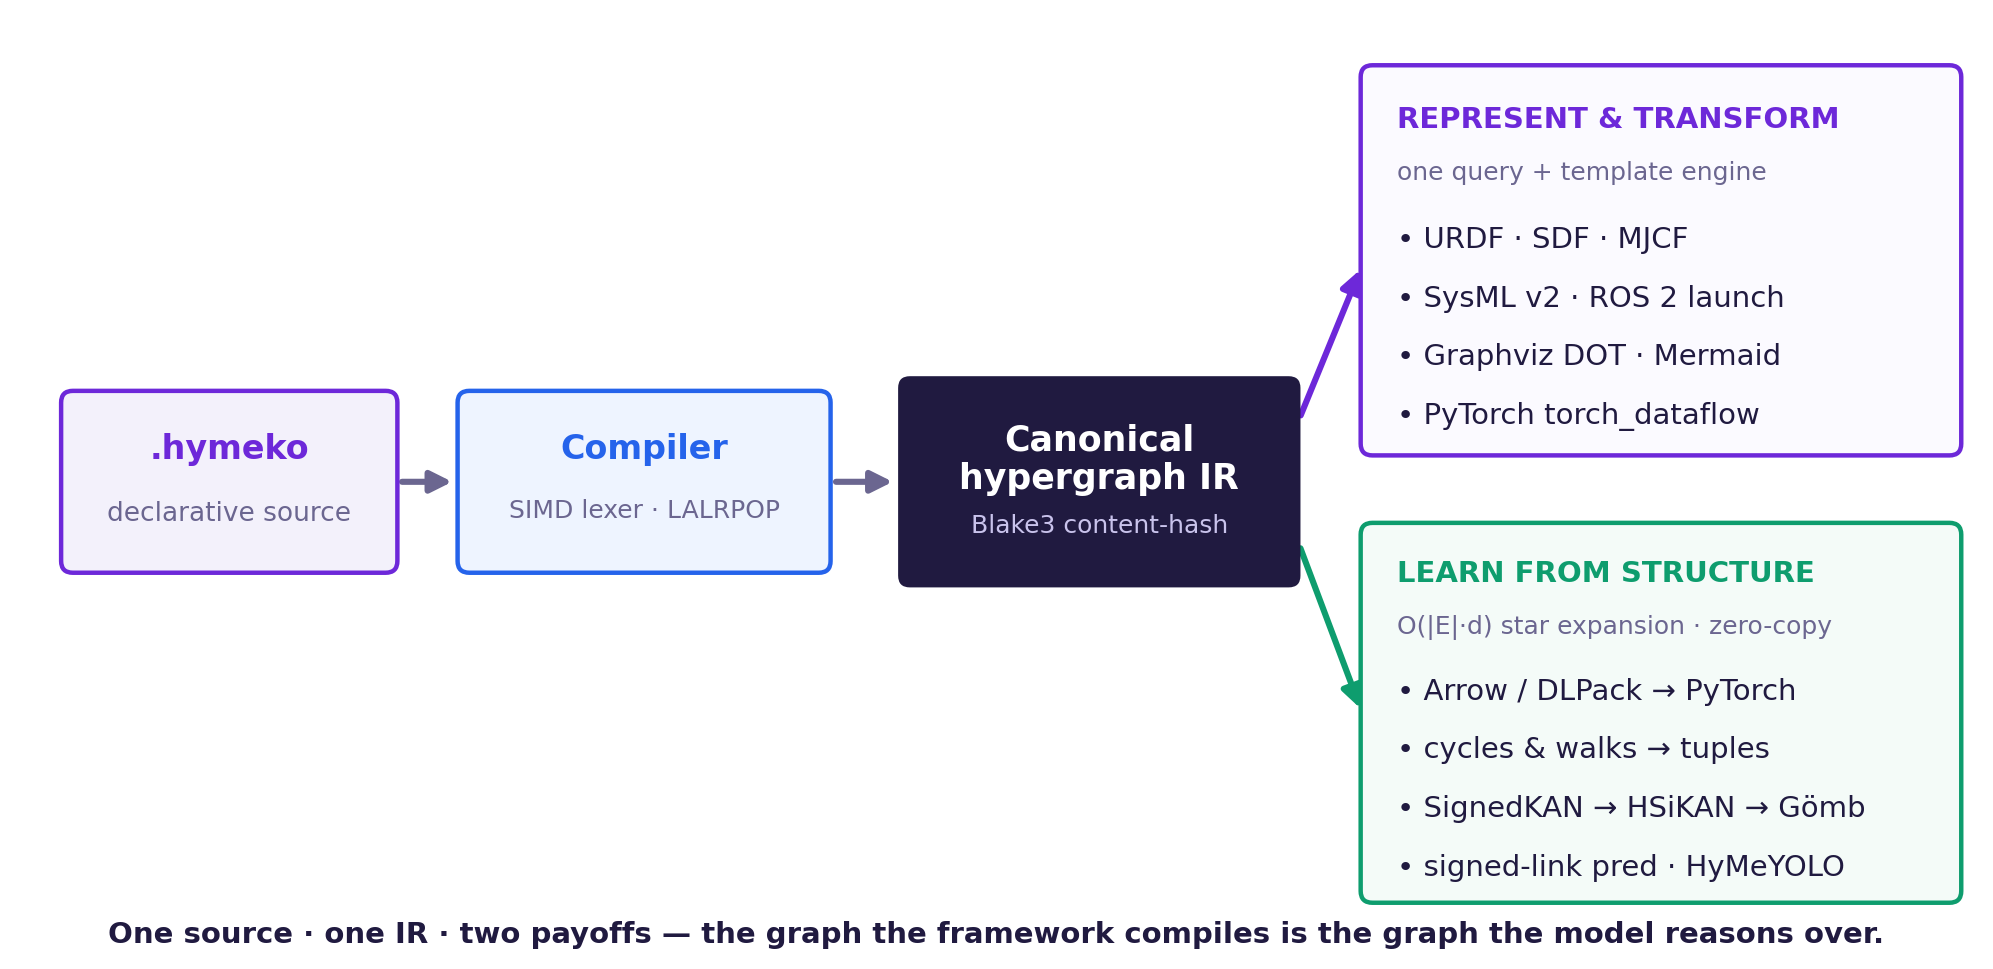
\includegraphics[width=.95\linewidth]{workflow.png}
\caption{The HyMeKo workflow: one source $\to$ one canonical IR $\to$ two payoffs (represent \& transform; learn from structure).}\end{figure}

\subsection*{How it works --- the pipeline}
\begin{enumerate}
\item \textbf{Author} --- a declarative \texttt{.hymeko} source; geometry, colours and vocabulary reused by reference, not duplicated.
\item \textbf{Compile} --- a SIMD lexer + LALRPOP parser produce one canonical hypergraph IR with a Blake3 content-hash identity.
\item \textbf{Represent} --- one query-and-template engine emits URDF, SDF, MJCF, SysML\,v2, ROS\,2 launch, DOT, Mermaid and a PyTorch module, cross-view consistent.
\item \textbf{Stream} --- the $O(|E|\,\bar d)$ star expansion goes zero-copy to PyTorch (Iceoryx2 / Arrow / DLPack); a topology-hash gate ($<100\,\mu$s) separates structure from weights.
\item \textbf{Enumerate} --- signed $k$-cycles and $k$-walks over the training edges become the structural tuples ($c_3\cdot c_4\cdot c_5\cdot w_2\cdot w_3$).
\item \textbf{Learn} --- SignedKAN $\to$ HSiKAN $\to$ G\"omb (Clifford-FIR $\to$ HSiKAN-CR $\to$ CPML) with Catmull--Rom splines, a per-edge CR highway (\texttt{edge\_cr}) and quaternion sign-attention.
\item \textbf{Audit} --- a leakage-audited strict protocol: the cycle pool never sees a test-edge sign; label-shuffle collapses to chance ($0.540$); 5-seed paired-$\Delta$.
\end{enumerate}

\section*{\color{accent}7.\quad Part I --- The framework}
\begin{itemize}
\item Declarative DSL with reuse by reference: a geometry (and colour) defined once, referenced by both visual and collision; the kinematics vocabulary imported once.
\item Canonical hypergraph IR with a Blake3 content-hash identity --- isomorphic descriptions share one fingerprint.
\item One query-and-template engine emits URDF / SDF / MJCF / SysML\,v2 / ROS\,2 / DOT / Mermaid / PyTorch --- no recompile per target.
\item Zero-copy bridge to PyTorch via Iceoryx2 / Arrow / DLPack, with a topology-hash gate ($<100\,\mu$s).
\end{itemize}

\begin{table}[h]\centering\small
\caption{Star vs.\ clique materialisation on the same 50-node / 50-edge / 0.30-density hypergraph --- the linear vs.\ quadratic cost of \S4 in numbers.}
\begin{tabular}{lrr}\toprule
Materialisation & Non-zeros & Extraction\\\midrule
Star \;$O(|E|\,\bar d)$ & 1{,}498 & 79.7 ms\\
Clique \;$O(|E|\,\bar d^{2})$ & 10{,}991 & 496 ms\\\bottomrule
\end{tabular}\end{table}

\begin{table}[h]\centering\small
\caption{Source size (characters), same robot. HyMeKo reuses geometry/colours by reference; URDF duplicates visual + collision. $^\dagger$The \emph{full} HyMeKo source also encodes joint-control interfaces, sensors and the Gazebo/ros2\_control deployment in \emph{one} file --- which plain URDF/MJCF cannot, so the kinematics-only MJCF figure is not a like-for-like comparison.}
\begin{tabular}{lrrr}\toprule
Kinematic structure & HyMeKo & URDF & MJCF\\\midrule
2-joint connection & 71 & 164 & 91\\
SCARA & 101 & 252 & 129\\
6-DoF arm (kinematics only) & 2{,}779 & 5{,}088 & 1{,}733\\
\addlinespace
6-DoF arm (full: $+$ control, sensors)$^\dagger$ & \textbf{6{,}134} & multi-file & mech.\ only\\\bottomrule
\end{tabular}\end{table}

\section*{\color{accent}8.\quad Part II --- Learning from structure}
\begin{itemize}
\item Enumerated signed $k$-cycles and $k$-walks become inductive features (tuples) --- structure as a prior.
\item SignedKAN $\to$ HSiKAN $\to$ G\"omb replaces fixed activations with learnable Kolmogorov--Arnold (Catmull--Rom) splines; HSiKAN adds an arity mixer, a per-edge Catmull--Rom highway (\texttt{edge\_cr}) and quaternion sign-attention.
\item G\"omb is a strict three-shell cascade --- Clifford-FIR (quaternion/multivector signed filter) $\to$ HSiKAN-CR $\to$ CPML --- with the cycle pool enumerated over training edges only.
\item A vision variant adds Clifford-FIR / quaternion machinery with Forman--Ricci curvature and Hodge decomposition ($\partial^2{=}0$, 1-homology, discrete Ricci flow).
\end{itemize}

\begin{figure}[h]\centering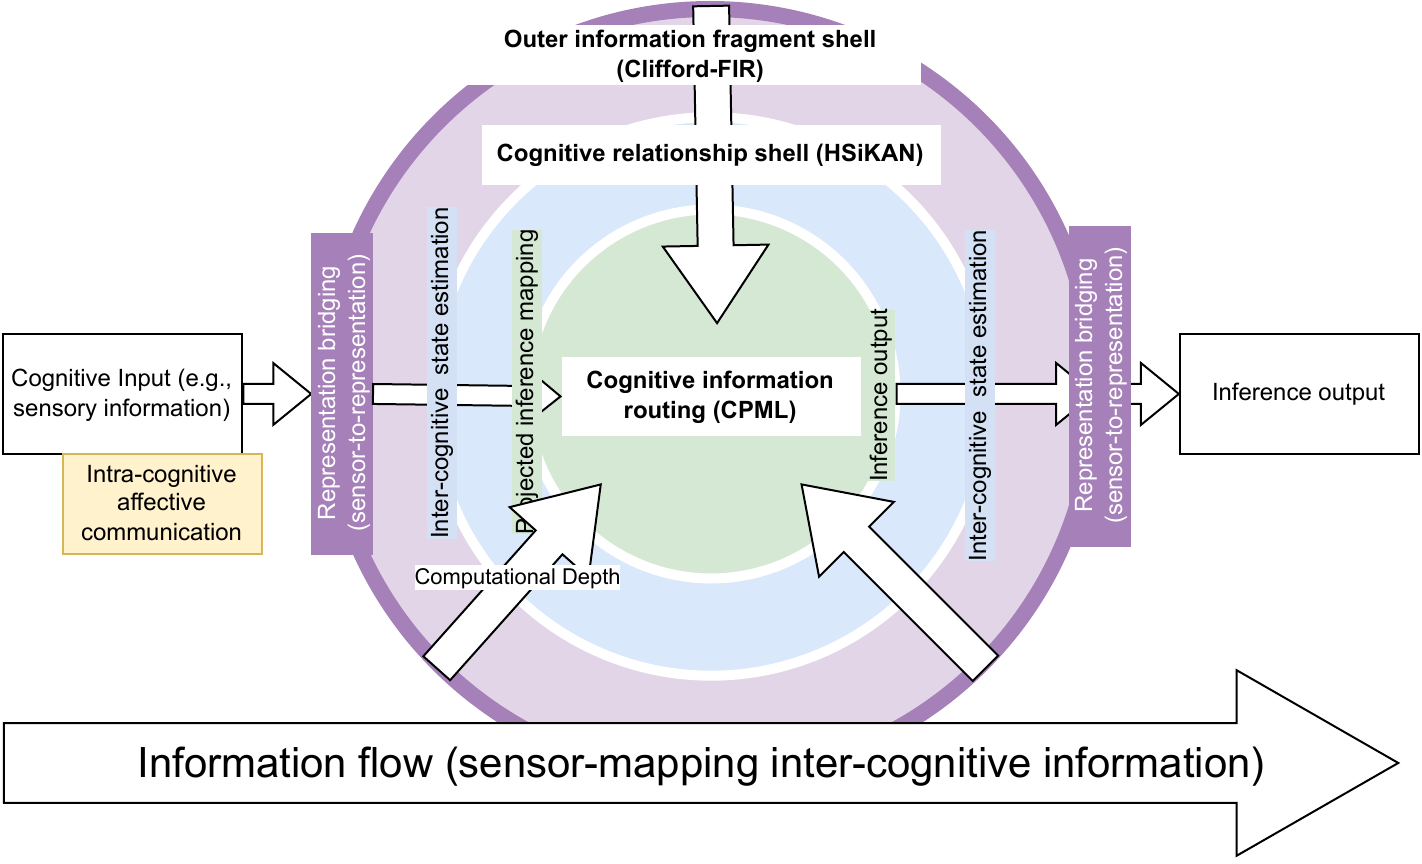
\includegraphics[width=.55\linewidth]{gomb.png}
\caption{The G\"omb structural-prior cascade (Clifford-FIR $\to$ HSiKAN-CR $\to$ CPML).}\end{figure}

\section*{\color{accent}9.\quad Key results (honest framing)}
\begin{itemize}
\item Competitive-to-leading at $\approx\!\tfrac14$ of the parameters, with the genuine lead on Epinions --- not a flat SOTA claim. (Under the transductive convention, tuned configs reach $0.996/0.993$ on Bitcoin.)
\item Efficiency: $\sim$30k parameters; the win is accuracy-per-parameter. Within-family forward gap (h4 vs.\ h16, same device) $\sim$3.5$\times$ on CPU, $\approx$1$\times$ on CUDA.
\item Transfer: HyMeYOLO reaches mAP$_{50}\approx0.90$ (a tie with a ReLU backbone); kinematics recovered from topology alone to $\approx$5\,cm.
\item Methodology: label-shuffle diagnostic (G\"omb $\to 0.540$ = chance); 5-seed paired-$\Delta$; every number maps to an on-disk artifact.
\end{itemize}

\begin{table}[h]\centering\small
\caption{Signed-graph link prediction, held-out test ROC-AUC (5-seed, G\"omb-strict). Baselines are published numbers.}
\begin{tabular}{lccc}\toprule
Dataset & \textbf{G\"omb-strict (ours)} & SGCN & SiGAT\\\midrule
Bitcoin-$\alpha$ & \textbf{0.897} & 0.929 & 0.903\\
Bitcoin-OTC & \textbf{0.915} & 0.942 & 0.932\\
Slashdot & \textbf{0.902} & 0.919 & ---\\
Epinions & \textbf{0.943} (FT 0.953) & --- & $\approx$0.95\\\bottomrule
\end{tabular}\end{table}

\section*{\color{accent}10.\quad New result --- Cayley-rotor embeddings (2026-06-16)}
A flat-parameter, inductive, leakage-free embedding: each item embedding is a learned rotation (a Clifford rotor via the Cayley map) of one shared reference on a sphere --- no per-node lookup table. It matches a growing-parameter baseline (DADSGNN) at $\sim$9--16$\times$ fewer parameters, and label-shuffle collapses it to chance ($\sim$0.50).

\begin{figure}[h]\centering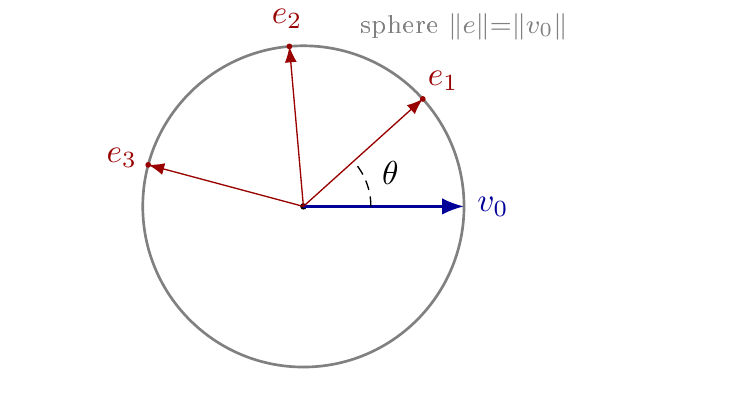
\includegraphics[width=.34\linewidth]{rotor.png}
\caption{The rotor embedding: each item is a rotation of one reference on a sphere; the angle is the similarity.}\end{figure}

\begin{table}[h]\centering\small
\caption{Signed-link test ROC-AUC, 5 seeds. Rotor is parameter-flat; the baseline grows. Source: \texttt{reports/rotor\_multiseed\_20260616.jsonl}.}
\begin{tabular}{lcccc}\toprule
Dataset & \textbf{Rotor AUROC} & \textbf{Rotor params} & DADSGNN AUROC & DADSGNN params\\\midrule
Bitcoin-$\alpha$ & \textbf{0.867 $\pm$ 0.011} & \textbf{15.8k} & 0.860 $\pm$ 0.011 & 142k\\
Bitcoin-OTC & \textbf{0.894 $\pm$ 0.006} & \textbf{15.8k} & 0.880 $\pm$ 0.007 & 209k\\
wiki\_elec & \textbf{0.885 $\pm$ 0.002} & \textbf{15.8k} & 0.896 $\pm$ 0.007 & 249k\\\bottomrule
\end{tabular}\end{table}

\section*{\color{accent}11.\quad Contributions \& contact}
\begin{itemize}
\item A canonical hypergraph infrastructure --- a DSL plus a content-hashed IR; one source, many targets.
\item A structural-prior learning family --- cycles and walks as inductive features (SignedKAN / HSiKAN / G\"omb), strictly leakage-audited. The same IR is both the engineering transform and the learning substrate.
\end{itemize}
Csaba Hajdu~~$\cdot$~~Kato Laboratory.\quad Code \& docs: \url{https://github.com/kyberszittya/hymeko_framework_rust}

\clearpage
\section*{\color{accent}12.\quad Slide-by-slide walkthrough}
This section mirrors the talk one slide at a time, so the handout can be read on its own after the seminar. Each entry says what the slide shows and why it is there; the conceptual slides (hypergraphs, balance, $k$-enumeration, leakage) are given a little more room, while the section dividers are kept to a single line.

\subsection*{Slide 1 --- Title}
The opening slide carries the talk title, the venue (Kato Laboratory), the speaker and the date. It also plants the single thread the whole talk follows: \emph{one substrate, two payoffs} --- the idea that the same hypergraph object can both describe a system and be learned from.

\subsection*{Slide 2 --- Contributions}
Two coupled contributions are stated before any detail, so the audience knows what to hold onto. (i) A canonical hypergraph \emph{infrastructure} --- a DSL and a content-hashed IR. (ii) A structural-prior \emph{learning} family that reads a graph's cycles. The point is that both rest on the \emph{same} IR, and the slide gives the four-block arc of the talk: problem $\to$ framework $\to$ learning $\to$ evidence.

\subsection*{Slide 3 --- HyMeKo, in brief}
A one-paragraph orientation for newcomers: HyMeKo is a Rust framework plus a small declarative language that compiles a hypergraph description into a canonical intermediate representation, and from that single representation both \emph{transforms} the structure into many target formats and \emph{learns} from it.

\subsection*{Slide 4 --- Why hypergraphs?}
The motivation. Many real relations bind more than two things at once ($n$-ary), and squeezing them into ordinary (pairwise) graphs both erases each relation's identity and inflates the representation. A $K_5$ illustration makes the cost concrete: turning one $k$-way relation into pairwise edges needs $\binom{k}{2}$ of them --- the $O(d^2)$ clique blow-up. The take-away the audience should leave with is simple: a $k$-ary relation is one object, and pairwise encoding both multiplies the edge count and forgets that those edges ever belonged together.

\subsection*{Slide 5 --- Typical hypergraphs}
A gallery of canonical examples --- the Fano plane, a generic hypergraph, the complete 3-uniform $K_4^{(3)}$, and a sunflower --- each with its hyperedges labelled and its \texttt{.hymeko} source shown alongside. The aim is to make ``hypergraph'' concrete and to show that these are real, compilable fixtures, not just pictures.

\subsection*{Slide 6 --- A hyperedge and its signed incidence}
Zooms in on a single hyperedge and shows its signed Levi/Berge incidence --- the bipartite ``star'' form with one hub node --- using green for $+$ and red for $-$. This is the representation everything downstream is built on.

\subsection*{Slide 7 --- One substrate, two payoffs}
The thesis slide. A single canonical IR serves both \emph{representation} (emitting many formats) and \emph{learning} (a structural prior), so that the graph the framework compiles is literally the graph the model reasons over --- not two separate artifacts that can drift apart.

\subsection*{Slide 8 --- What HyMeKo describes}
Surveys the domains the substrate covers in practice: robot mechanisms and kinematics, model-based systems engineering / SysML, signed social graphs, and neural-network dataflow --- evidence that the abstraction is general, not bespoke to one field.

\subsection*{Slide 9 --- Goals at two levels}
Separates the goals into the \emph{language} level (an ergonomic, reusable DSL) and the \emph{infrastructure} level (a fast compiler, a canonical IR, and a zero-copy runtime), so the contributions can be judged on each.

\subsection*{Slide 10 --- The HyMeKo workflow --- at a glance}
A single-page map of the whole system: a \texttt{.hymeko} source compiles through the lexer/parser to the canonical IR, which then fans out to the two payoffs --- represent \& transform on one side, learn from structure on the other. It is the mental model for everything that follows.

\subsection*{Slide 11 --- Part I divider}
A section divider that opens the framework half of the talk.

\subsection*{Slide 12 --- A declarative language for hypergraphs}
Introduces the DSL: hyperedges are first-class, nodes nest into hierarchical paths, arcs carry $+/-$ signs and role tags. A \emph{compilable} \texttt{robot.hymeko} example shows the key ergonomic idea --- a geometry (and colour) is defined once and \emph{referenced} by both the visual and the collision, rather than duplicated.

\subsection*{Slide 13 --- From source text to a hypergraph IR}
Walks through the compiler: a SIMD-accelerated lexer and an LALRPOP (LR(1)) parser produce a canonical IR whose nodes carry a Blake3 content-hash identity (so isomorphic descriptions share one fingerprint), with symbol interning and the star/clique expansions available on demand.

\subsection*{Slide 14 --- Star vs clique: the efficiency argument}
Quantifies $\S4$'s linear-vs-quadratic point on one fixed 50-node / 50-edge / 0.30-density hypergraph: the star expansion needs 1{,}498 non-zeros and 79.7\,ms, the clique expansion 10{,}991 and 496\,ms. The two tensor heatmaps make the density difference visible.

\subsection*{Slide 15 --- A zero-copy bridge to the GPU}
Explains how the star expansion streams into PyTorch with no copying --- via Iceoryx2 shared memory, Apache Arrow and DLPack --- and how a topology-hash gate ($<100\,\mu$s) tells structural updates apart from weight streams, so only what changed is re-sent.

\subsection*{Slide 16 --- Query-driven transforms: one graph, many targets}
Shows the query-and-template engine emitting URDF, SDF, MJCF, SysML and a PyTorch module from the one IR. The $N\times M$ pairwise-converter problem collapses to a hub-and-spoke, and every emitted view is guaranteed consistent with the others.

\subsection*{Slide 17 --- How compact is the DSL?}
A character-count comparison (HyMeKo vs URDF vs MJCF) on a 6-DoF arm, with the honest framing developed live: HyMeKo wins by reusing geometry/colours by reference where URDF duplicates visual + collision, and the full \emph{deployable} system is one \texttt{.hymeko} file versus a multi-file ROS/Gazebo bundle. A screenshot shows the generated robot simulated in MuJoCo.

\subsection*{Slide 18 --- Built like a system, not a script}
The engineering discipline behind the code: a SysML\,v2 model, a \texttt{CORE.YAML} protection contract that marks the read-only core, and a plan-first workflow --- evidence that the framework is maintained as a system.

\subsection*{Slide 19 --- Part II divider}
A section divider that opens the science half of the talk.

\subsection*{Slide 20 --- From structure to inductive prior}
The hinge from Part I to Part II: a graph's cycles and walks are turned into tuples that act as structural features, and the cycle-arity \emph{compass} is shown as a fingerprint of a mechanism family. Notably the model itself is also expressed in \texttt{.hymeko}.

\subsection*{Slide 21 --- The model family: SignedKAN, HSiKAN, G\"omb}
Lays out the progression of models and names the deployable configuration --- Clifford-FIR $\to$ HSiKAN-CR $\to$ CPML --- so the later detailed slides have a map to sit in.

\subsection*{Slide 22 --- G\"omb: a strict structural-prior cascade}
Details the three shells (Clifford-FIR $\to$ HSiKAN-CR $\to$ CPML) and the one design choice that makes it honest: the cycle pool is enumerated over \emph{training} edges only, so a test edge's sign can never leak in --- a label-shuffle collapses it to chance.

\subsection*{Slide 23 --- What is k-enumeration? Why HSiKAN needs it}
Explains the structural features themselves: enumerating signed $k$-cycles and $k$-walks of each arity, with graphical examples of a closed cycle and an open walk. It also explains why this is the bottleneck and how it is bounded --- per-vertex top-$k$ scoring and per-arity caps. In short, $k$-enumeration is how raw topology becomes a fixed-width feature that the spline layer can consume, and the caps are what keep it tractable on dense graphs.

\subsection*{Slide 24 --- Inside HSiKAN}
Opens the middle shell: the Catmull--Rom spline activation, the mixed-arity layers fused by an arity mixer, quaternion sign-attention, and the per-edge Catmull--Rom highway (\texttt{edge\_cr}) that is the strong reference configuration.

\subsection*{Slide 25 --- HSiKAN, learned: alpha-k regime and ROC}
Shows real inference output rather than a schematic: the learned arity-weight vector $\alpha_k$ (which cycle lengths the model relies on) and the ROC curve with its AUROC.

\subsection*{Slide 26 --- Clifford-FIR and quaternion machinery}
The outer shell: parallel Clifford-FIR filter banks built on the \texttt{hymeko\_clifford} autograd backend (multivectors, blade products, a $(p,q)$ metric), with Forman curvature, Hodge decomposition and Bochner --- framed through a V1$\to$V4$\to$IT analogy.

\subsection*{Slide 27 --- Signed-graph link prediction results}
The headline results: held-out 5-seed ROC-AUC across datasets under the G\"omb-strict protocol, next to published baselines, presented as a table and a chart with the honest framing (competitive-to-leading at a fraction of the cost, a genuine lead on Epinions, not a flat SOTA claim).

\subsection*{Slide 28 --- SOTA range --- at a fraction of the cost}
The efficiency story: $\sim$30k parameters and a win measured in accuracy-per-parameter, the within-family width gap (h4 vs h16), and a note on the Komondor supercomputer used for the large multi-seed runs.

\subsection*{Slide 29 --- New result: Cayley-rotor embeddings}
The newest result: a flat-parameter, inductive, leakage-free embedding where each item is a learned rotation of one shared reference on a sphere (a Clifford rotor via the Cayley map). It matches the growing-parameter DADSGNN baseline at 9--16$\times$ fewer parameters, and label-shuffle collapses it to chance.

\subsection*{Slide 30 --- What is leakage? Why it matters}
A teaching slide on the failure mode the protocol guards against: transductive $\sigma$-leakage, where a model scores well by secretly reading test-edge signs through the structure rather than predicting them. Concretely: if the cycle pool is built over all edges, a cycle through a held-out edge can already ``see'' its sign, and a high score then measures memorisation, not generalisation --- which is why the next slides are about ruling this out.

\subsection*{Slide 31 --- Honesty as a protocol}
States the evaluation stance: a strict protocol in which every reported number maps to an on-disk artifact, and claims are framed conservatively.

\subsection*{Slide 32 --- How we know it isn't leakage}
The evidence for the previous slide: re-training with the training-edge signs shuffled drives G\"omb to $0.540$ (chance), which proves its skill comes from genuine structure, not from a memorised table. The logic is a control experiment: destroy the structure (shuffle the signs) and the skill must vanish if it was structural --- it does, falling to the chance line, so the signal the model uses is the balance pattern, not a leaked label.

\subsection*{Slide 33 --- HyMeYOLO: detections on Cluttered MNIST}
The vision transfer: a hypergraph-convolution detector finding digits in Cluttered MNIST, reaching mAP$_{50}\approx0.90$ --- an honest statistical tie with a ReLU backbone, presented as an \emph{approach} to hypergraph convolution, on a Ricci-curvature / Hodge backbone.

\subsection*{Slide 34 --- The bridge}
Ties the two halves together: \texttt{.hymeko} structure $\to$ IR $\to$ sparse incidence tensor $\to$ structural-prior model, i.e.\ one DSL describes the robot and the network that reasons about it. The embedded MuJoCo video shows graph-only kinematics tracking the simulator.

\subsection*{Slide 35 --- Live demo: UR5e grasping context}
The live, on-robot-stack demo (MDPI Technologies Tier-1): one launch command brings up Gazebo + UR5e + MoveIt\,2 + RViz\,2 plus the HyMeKo grasping-context node, which loads \texttt{hymeko\_robot.hymeko}, evaluates 6 signed hyperedges at 10\,Hz and republishes contextual outputs as ROS topics. The slide pairs the architecture schematic with the recorded MoveIt demo.

\subsection*{Slide 36 --- Publications \& submissions (2026)}
The publication portfolio shown as a one-substrate-many-outputs fan, situating the infrastructure paper and the HSiKAN work-in-progress within the wider body of work.

\subsection*{Slide 37 --- Future work}
The near-term programme: finishing the $\sigma$-masked strict protocol, a runnable \texttt{.hymeko}$\to$\texttt{torch.nn} round-trip, broader transform targets, larger signed-graph and vision corpora, the HSMM$\to$FPGA path, and an in-browser authoring editor.

\subsection*{Slide 38 --- Minimum demo \& collaboration}
The smallest end-to-end demo that proves the thesis, and a concrete collaboration ask: robot-structure learning, encoding morphology and task in HyMeKo and testing whether structural priors help control.

\subsection*{Slide 39 --- Acknowledgements}
Thanks to Kato Laboratory for hosting the seminar and to the collaborators and co-authors.

\subsection*{Slide 40 --- Conclusion \& outlook}
Recaps the single idea --- one substrate, two payoffs --- and the bridge between describing a system and learning from it, then looks ahead.


\end{document}
